

This chapter reviews some of the theoretical concepts relevant to the subsequent physics analysis. Aspects of the SM relevant to this analysis are introduced. The importance of the top quark within the SM is then discussed. Then, predictions for the production properties of top quarks at the LHC are reviewed.

\section{The Standard Model}

The SM of particle physics is one of the most precisely tested and successful theories in the history of physics~\cite{peskin}. The theory represents the best current understanding of the fundamental behavior of subatomic particles and provides the framework for particle physics predictions. Most predictions of the SM have been verified and found to be self-consistent up to the Planck scale ($10^{15-19}$ \gev). A thorough treatment of the theoretical framework can be found in textbooks such as Refs.~\cite{peskin,halzen1984quarks,PDG}.

The SM uses the mathematical framework of Quantum Field Theory (QFT) to describe two kinds of particles, fermions and bosons. Fundamental interactions between these particles can be derived from the conservation of a symmetry called gauge invariance. This general principle maps conserved quantities to the invariance of the Lagrangian under some transformation, an example of Noether's theorem. The SM provides a unified description of the strong, weak and electromagnetic forces, but does not (yet) include gravity. The symmetry group of the SM is $SU(3)\times SU(2)\times U(1)$.
\subsection{Particles of the SM}

Tables~\ref{t:pspincharge}-\ref{t:pmass} summarize the properties of the fundamental particles of the SM described below.

Fermions are spin-$\frac{1}{2}$ point-like particles that form ordinary matter. The two types of fermions are known as leptons and quarks. The three lepton generations, each with a charged lepton and a neutrino, interact via the electroweak force. The three quark generations, each with an up-type and down-type quark, interact via both the electoweak force and the strong force. The strong force combines quarks into composite particles. Three such quarks form a baryon, while two quarks form a meson. Each fermionic generation is identical to the first, except for mass. 

Bosons are particles with integer spin that mediate interactions between particles. Each gauge boson corresponds to a different fundamental force, and the range each force is inversely related to the boson mass.
\begin{description}
\item[Electromagnetic (EM) force] mediated by the massless and chargeless photon ($\gamma$). Since the photon is massless, the range of the EM force is infinite. The EM force is responsible for many common interactions, such as radiation of photons from excited atoms.
\item[Weak force] mediated by the $W^{\pm}$ and $Z^{0}$ bosons and is responsible for nuclear reactions such as beta decay .
\item[Strong force] mediated by gluons ($g$) is responsible for the formation of protons and neutrons. The quarks are the only fermions that interact strongly. 
\end{description}
\begin{table}
\begin{tabular}[b]{|l||ccc|c|c|}
\hline
           & \multicolumn{3} {c|} {particles} & spin & electric charge \\
\hline
\hline
               & $(u,d)_L$ & $(c,s)_L$ & $(t,b)_L$ & $(\frac{1}{2},\frac{1}{2})$ & $(+\frac{2}{3},-\frac{1}{3})$ \\
Quarks         & $u_R$     & $c_R$     & $t_R$     & $\frac{1}{2}$               & $+\frac{2}{3}$                \\
               & $d_R$     & $s_R$     & $b_R$     & $\frac{1}{2}$               & $-\frac{1}{3}$                \\
\hline
\multirow{2} {*} {Leptons} & $(\nu_e, e^-)_L$ & $(\nu_{\mu},\mu^-)_L$ & $(\nu_{\tau}, \tau^-)_L$ & $(\frac{1}{2},\frac{1}{2})$ & (0,-1) \\
                           & $e^-_R$          & $\mu^-_R$             & $\tau^-_R$               & $\frac{1}{2}$               & -1     \\
\hline
                           & \multicolumn{3} {c|} {$g$}               & 1 & 0 \\
Gauge bosons               & \multicolumn{3} {c|} {$W^{\pm}$ and $Z$} & 1 & $\pm$1 and 0 \\
                           & \multicolumn{3} {c|} {$\gamma$}          & 1 & 0 \\
\hline
Scalar boson               & \multicolumn{3} {c|} {$H$} & 0 & 0 \\
\hline 
% 
\end{tabular}
\caption{Spin and charge of particles in the SM.}
\label{t:pspincharge}
\end{table}
\begin{table}

\begin{tabular}[b] {|l|l|l|}
\hline
& Particle & Mass  \\
%%%%%%%%%%%%%%%%%%%%%%%%%%%%
\hline
\hline
\multirow{3} {*} {Leptons} & $e$ & 0.511 MeV  \\
& $\mu$ & 105 MeV \\
& $\tau$ & 1777 MeV \\
\hline \hline
 \multirow{3} {*} {Gauge bosons} & $W^{\pm}$ & 80.2 GeV \\
& $Z$ & 91.19 GeV  \\
\hline
& $H$ & 126 GeV \\
\hline \hline
 \multirow{3} {*} {Quarks} & up ($u$) & 1.7-3.3 \mev \\
& down ($d$) & 4.1-5.8 \mev  \\
\hline
& charm ($c$) & 1.18-1.34 \gev  \\
& strange ($s$) & 70-120 \mev \\
\hline
& top ($t$) & $173.34 \pm 0.76$  \gev  \cite{ATLAS:2014wva}\\
& bottom ($b$) & $4.18 \pm 0.03$ \gev \\
\hline \hline
\multirow{3} {*} {Hadrons} & $p$ & 938 MeV\\
& $n$ & 939 MeV  \\
& $\pi^{\pm}$ & 139.6 MeV \\
& $\pi^0$ & 135.0 MeV  \\
\hline
\end{tabular}
\caption{Mass of particles in the SM, taken from Ref.~\cite{PDG}.}
\label{t:pmass}
\end{table}

Discovered in 2012, the Higgs boson is the final particle in the SM. In order to explain the mass difference between the photon and electroweak bosons, the symmetry between the EM and weak forces must be broken. The Higgs field interacts with the electroweak gauge bosons to provide masses while preserving the local gauge invariance of the SM.

At low energy, the EM and weak forces appear distinct. Above the unification energy ($\sim 100 $\gev), the EM and weak forces are unified into a single interaction known as the electroweak interaction. The corresponding symmetry group is $SU(2)\times U(1)$, where $SU(2)$ represents the weak force and $U(1)$ represents the EM force. 


\subsection{Quantum chromodynamics}
Quantum chromodynics (QCD) is a gauge theory which interactions between quarks via the strong force. The six flavors of quarks ($u,d,s,c,b$ and $t$) each carry a conserved quantum number called color, which is analogous to electric charge in QED. Neither quarks nor gluons can exist as free particles. Instead, color-neutral combinations of quarks, anti-quarks and gluons called hadrons are observed. The quark and gluon consituents of a hadron are traditionally called partons.

The QCD Lagrangian for the interaction between two quarks $i$ and $j$ can be written as~\cite{PDG}:
\begin{eqnarray}
\mathcal{L}_{QCD} = \bar{\psi}_i(i\gamma^{\mu}\partial_{\mu}\delta_{ij} - g_s\gamma^\mu t^C_{ij}\mathcal{A}^C_\mu -m\delta_{ij})\psi_j -\frac{1}{4}G^{A}_{\mu\nu}G^{\mu\nu}_A,\\
\mbox{where } G^A_{\mu\nu} \equiv \partial_\mu \mathcal{A}^A_{\nu}-\partial_\nu \mathcal{A}^A_{\mu} - g_s f_{ABC} \mathcal{A}^B_{\mu} \mathcal{A}^C_{\nu},
\end{eqnarray}
where repeated indices are summed over, $\gamma^{\mu}$ are the Dirac $\gamma$ matrices. ${\psi}_i$ is the quark-field spinor, where the color index $i$ can correspond to one of three ($N_C$) quark flavors. $\mathcal{A}^{B}_{\mu}$ represents the gluon fields, where $C$ runs from 1 to $N_C^2-1=8$, corresponding to eight types of gluons. $t^{A}$ are the eight $3 \times 3$ generating matrices of $SU(3)$ and $f_{ABC}$ the group structure constants of $SU(3)$. The fundamental parameters are the coupling $g_s$ and the quark masses $m$.

The structure of the Lagrangian predicts three types of vertices: a quark-antiquark-gluon ($q\bar{q}g$) vertex proportional to $g_s$, a three gluon vertex  proportional to $g_s$, and a four gluon vertex proportional to $g_s^2$. Since gluons carry color charge, they can directly couple to other gluons, unlike other bosons. These self-interaction vertices mean that QCD has divergent terms that are not found in other SM sectors.
\subsubsection{Running of the coupling}

In the context of perturbative QCD, \emph{order} refers to the degree of $\alpha_S$ used in the calulation: leading order (LO), next-to-leading order (NLO)next-to-next-to leading order (NNLO), etc. Pertubative QCD calculations at NLO and beyond necessarily involve these divergent quark and gluon loops. These divergences must be removed in order to obtain a physical result. In order to remove the divergences, the strong coupling constant must be ``renormalized'' and expressed as a function of an (unphysical) renormalization scale $\mu_R$. Notably, QCD predictions change depending on the scale of the probe. This is sometimes referred to as the ``running'' of the coupling constant. Predictions for a given process are evaluated with $\mu_R$ as close to the momentum transfer $Q$ as possible, so that $\alpha_s(\mu_R \simeq Q)$ gives the effective strength of the strong force in that particular process. 

The strong coupling constant $\alpha_S \equiv g_s^2/4\pi$ is related the renormalization scale $\mu_R$ by the renormalization group equation (RGE):
\begin{equation}
\mu_R^2 \frac{\alpha_S}{\mu^2_R} = \beta \left( \alpha_S \right) = -\left( b_0\alpha^2_S + b_1\alpha^3_S + b_2\alpha^4_S + \dotsb \right)
\label{eq:rge}
\end{equation}
where the coefficients $b$ are called the beta-function coefficients and depend on the number of quark colors. The values of the beta coefficients up to $b_3$ can be found in Ref.~\cite{vanRitbergen:1997va}. 

Figure~\ref{fig:alphas} shows the NLO QCD prediction for $\alpha_S$ as a function of $Q$, as well as several experimentally measured values of $\alpha_S$ for discrete energy scales. Experimental measurement agrees very well with the theoretical predictions. The negative sign on the right side of Eqn.\ref{eq:rge} means that the strong coupling becomes weaker as the scale increases: $\alpha_S \sim 0.1$ for momentum transfers $100 \gev \lesssim Q \lesssim 1 \tev$. This is the origin of the previously mentioned asymptomic freedom, which allows partons to be considered approximately free at high energy. The divergence of the coupling constant at low energy results in the formation of stable hadrons and is called ``confinement.''

\begin{figure}[h]
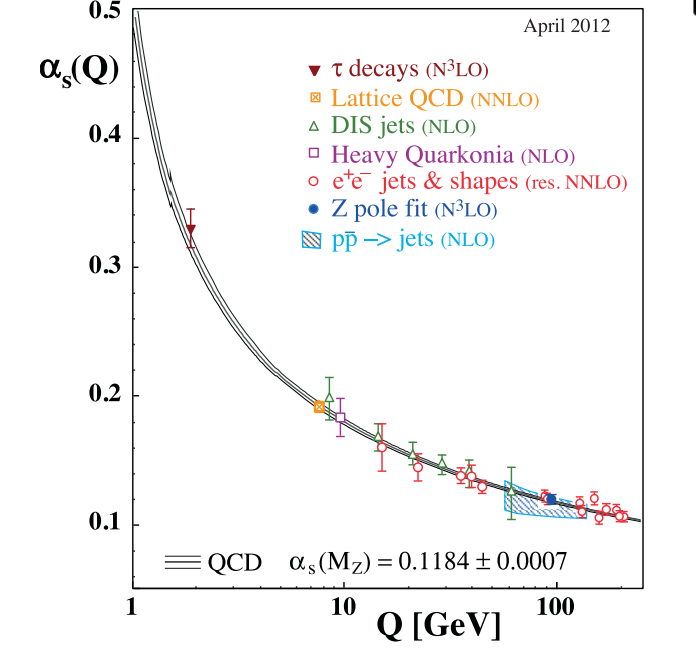
\includegraphics[width=\textwidth]{fig/thry/RunningAlpha.png}
\caption{Summary of measurements of $\alpha_S$ as a function of the respective energy scale, $Q$, from Ref.~\cite{PDG}. The respective degree of QCD perturbation theory used in the extraction
of $\alpha_S$ is indicated in brackets (NLO: next-to-leading order; NNLO: next-to-next-to leading order; res. NNLO: NNLO matched with resummed next-to-leading logs;
N3LO: next-to-NNLO).}
\label{fig:alphas}
\end{figure}
\subsubsection{Parton distribution functions}

In high energy scattering, the proton cannot be modeled as three free non-interacting quarks in a bag; the internal partonic structure of the proton must be considered~\ref{PDG,Campbell:2006wx}. The three \emph{valence} quarks exist in a sea of virtual quark-antiquark pairs that arise from the gluons holding the quarks together. All of these partons contribute to the internal structure of the proton. The proton can be modeled as a collection of these partons that are each carrying a fraction $x$ of the proton's momentum. The \emph{Parton Distribution Function} (PDF) describes the internal proton structure via normalized momentum distribution functions of the constituent partons

 Since the PDFs deal with the non-perturbative regime of QCD, PDFs must be determined by global fits to experimental measurements of deep inelastic and other hard-scattering processes. PDFs derived from measurements of one process can be used for predictions in a different process. For example, positron-proton scattering data from the HERA experiment can be used to make predictions for proton-proton collision at the LHC. One common PDF set used at the LHC, called MSTW, is shown in Figure~\ref{fig:mstw}.

PDF measurements depend on the scale of the hard probe, so theoretical calculations are needed to evolve the PDFs between experimental data points. The differential equations governing the $\mu^2$ dependence of the PDFs are called the DGLAP equations and are derived in Ref.~\cite{Altarelli:1977zs}. Much like the RGE introduces an arbitrary $\mu_R$, the DGLAP equations introduce a factorization scale $\mu_F$ to absorb the divergences from soft parton emissions. To avoid unnaturally large logarithms in the pertubative expansion,  $\mu_F$ and $\mu_R$ are usually assumed to be equal and of the order of the typical momentum scales of the hard scattering process. The theoretical uncertainty from the arbitrary choice of $\mu_F$ and $\mu_R$ is usually evaluated by repeating the calculation with the scale doubled and halved.
\begin{figure}
\centering
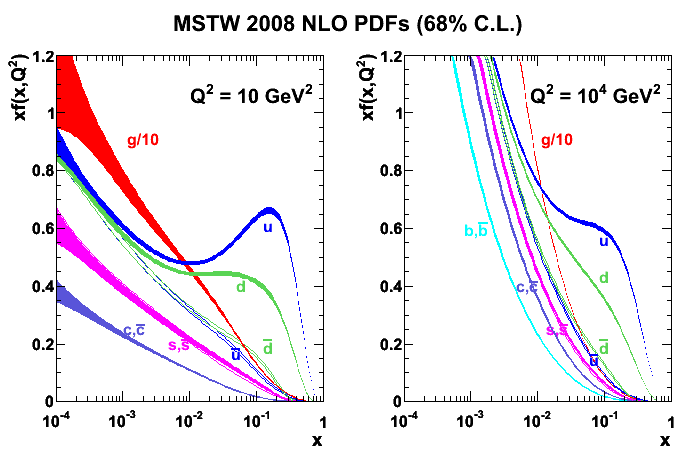
\includegraphics[width=0.8\textwidth]{fig/thry/mstw.png}
\caption{MSTW 2008 NLO PDFs at $Q^2= 10 \gev^2$ and $Q^2= 10^4 \gev^2$~\cite{mstw}.}
\label{fig:mstw}
\end{figure}


\subsubsection{Factorization}


Because of the scale dependence of QCD, interactions can be separated into two regimes, with the transition around the QCD confinement scale, $\Lambda_{QCD} \sim 200$ MeV, the energy at which QCD because non-perturbative. At low energy, $\alpha_S$ is of order unity, so perturbative expansion is not possible. The quarks are bound together by soft gluon emissions into a proton. At scales far above the QCD confinement scale, the partons can be considered free objects and can be treated with perturbative expansion.

The hard scatter interaction with momentum transfer $Q$ occurs on a time scale that goes as $\tau \sim 1/Q$ which is much larger than the time scale of interactions between protons $\tau \sim 1/\Lambda_{QCD}$. This fact allows high energy proton collisions to be \textit{factorized} into two independent processes: the PDF, which a phenomelogical description of the momentum distribution among the partons inside the proton which depends only on the momentum scale, and the partonic cross section $\hat{\sigma}$, which uses perturbative QCD to determine the calculates the scatter of the hard probe from one of the free partons inside the proton.


Specifically, the hadronic cross-section for a particular process can be written the weighting of the subprocess cross section with the PDFs $f_{q/A}(x)$ extracted from deep inelastic scattering experiments\cite{Campbell:2006wx}:
\begin{eqnarray}
\sigma(AB\rightarrow X) &=& \int dx_a dx_b \,f_{a/A}(x_a,\mu_F^2) f_{b/B}(x_b,\mu_F^2) \hat{\sigma}_{ab \rarrow X} \nonumber \\
&=& \int dx_a dx_b \,f_{a/A}(x_a,\mu_F^2) f_{b/B}(x_b,\mu_F^2) \,\times\,[\sigma_0 + \alpha_{S}(\mu_R^2)\sigma_1 + ...]
\label{eq:ab}
\end{eqnarray}
which is diagramatically represented in Figure~\ref{fig:factorize}. The partonic cross-section can be pertubatively expanded in powers of the strong coupling constant $\alpha_S$ for some renormalization scale $\mu_R$. The PDF $f_{a/A}(x_a,\mu_F^2)$ gives the probability that a proton with momentum $p_A$ contains a parton $a$ with momentum $p_a$. This function depends only on the fraction of the proton momentum distributed to parton $a$, $x_a \equiv p_a/p_A$, and the factorization scale $\mu_F$. 
\begin{figure}[h]
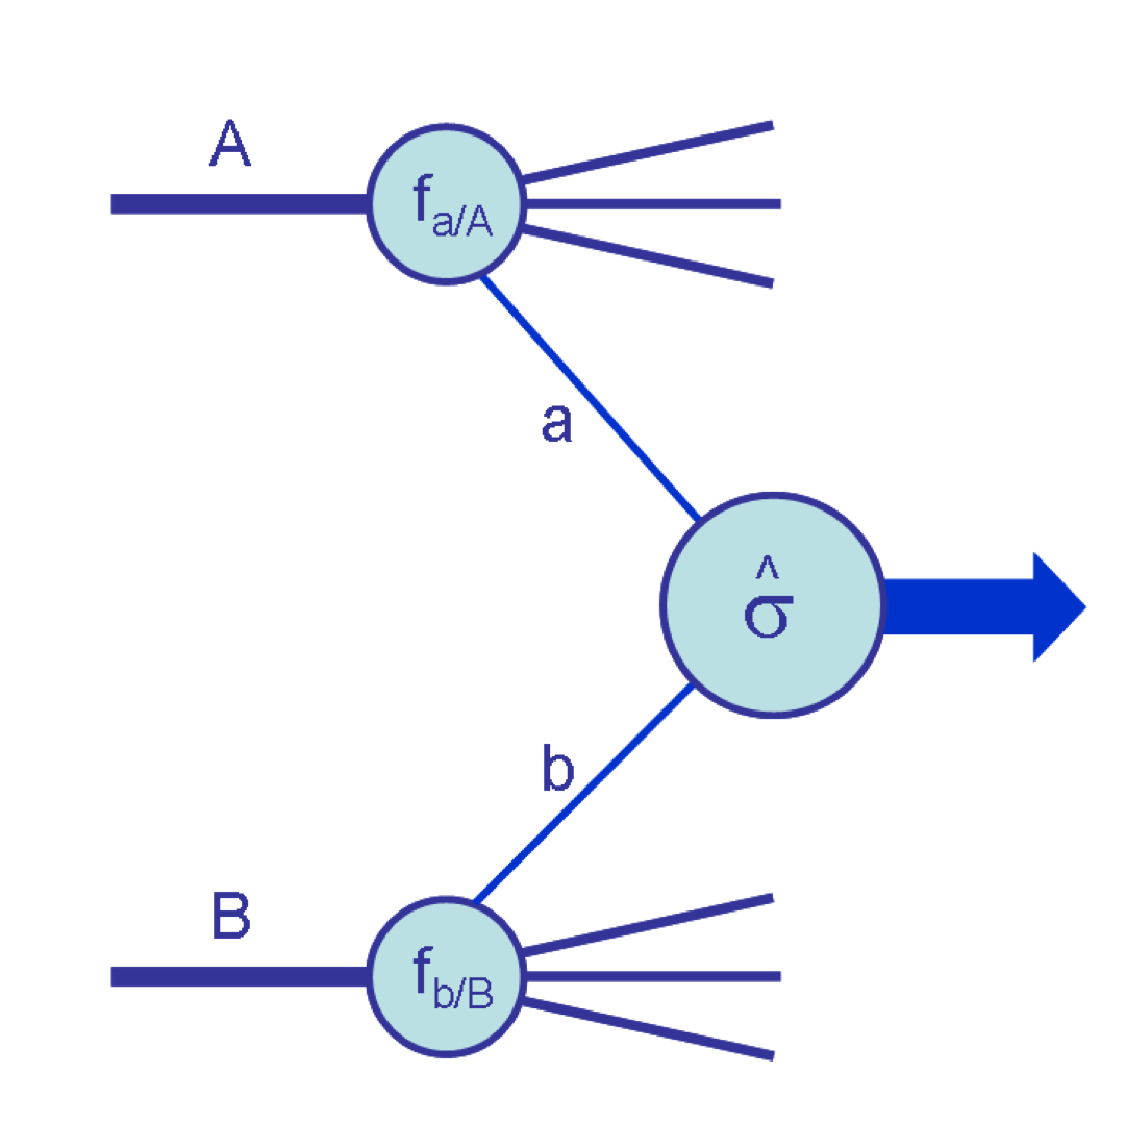
\includegraphics[width=0.9\textwidth]{fig/thry/Factorize.pdf}
\caption{Diagram from Ref.~\cite{Campbell:2006wx} illustrating the structure of a generic hard scattering process of two incoming partons $A$ and $B$ with PDFs $f_{a/A}$ and $f_{b/B}$.}
\label{fig:factorize}
\end{figure}










\section{Top quark physics}
The top quark was first discovered at Fermilab in 1995~\cite{Abe:1995hr}\cite{Abachi:1995iq}. As the heaviest known fundamental particle, the top quark is an important probe of the SM and extensions of the SM. Before the Large Hadron Collider (LHC), the Tevatron provided the only experimental observation of the top. The LHC produces a top quark every few seconds, about a hundred times more frequently than the Tevatron. This signifigant increase in statistics allows precision measurements of the top at the LHC, which is sometimes called a ``Top Factory.'' 

Because of its large mass, the top quark plays a special role in the SM. The top mass is about the same as a gold atom nucleus, 40 times larger than the next heaviest quark and $10^5$ times heavier than the lightest quark. The mass of the top quark has been precisely measured in different decay channels at both the LHC and the Tevatron. Figure~\ref{fig:topmass} shows a recent summary of these measurements, which can be combined to give a world average of $173.34 \pm 0.76$ for the top quark mass.

 The top has a very short lifetime ($\sim 5 \e{-25}$ s), so it is the only quark that decays before it can form a hadron with other quarks. This unique property means that the top is the only ``bare'' quark that can be accessed at the LHC. The top is also the only quark with Yukawa coupling to the Higgs boson of order unity. Thus, accurately measuring its properties (mass, coupling, cross section, branching ratios) provides an important information about Quantum Chromodynamics (QCD), the SM description of interactions between quarks via the strong force. 



\begin{figure}
\centering
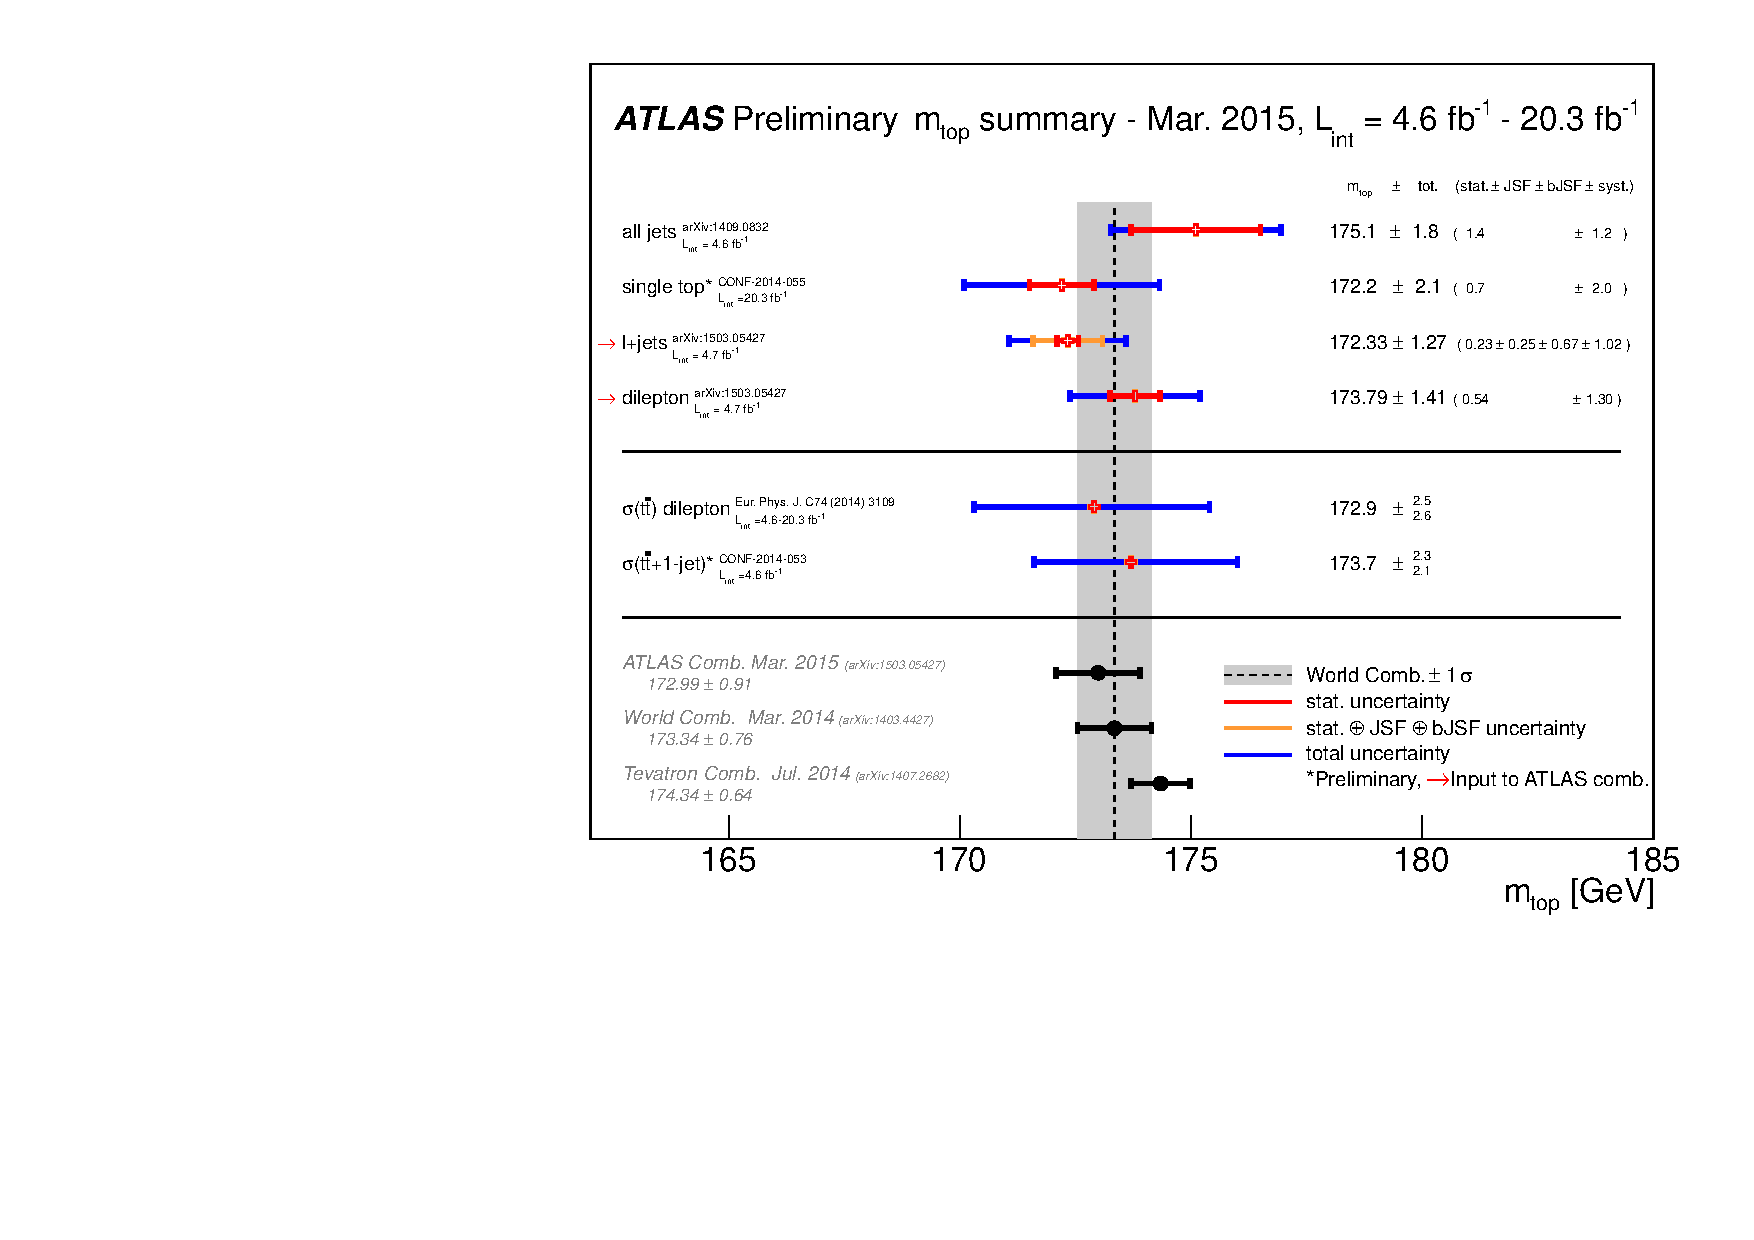
\includegraphics[width=0.8\textwidth]{fig/thry/mtopSummaryAll.pdf}
\caption{Summary of the ATLAS direct $m_{top}$ measurements. The results are compared with the ATLAS, Tevatron and Tevatron+LHC $m_{top}$ combinations. For each measurement, the statistical uncertainty, the sum of the remaining uncertainties are reported separately.}
\label{fig:topmass}
\end{figure}

\subsection{Top quark production at the LHC}

In $pp$ collision at the LHC, top quarks are mostly produced in pairs through the leading order QCD processes  $gg \rightarrow \ttbar$ and $q\bar{q} \rightarrow \ttbar$. The Feynman diagrams for these processes are shown in Figure~\ref{fig:ttdiag}. At Tevatron with $p\bar{p}$ collisions, \ttbar production was dominated by quark annihilation ($\sim 85$\%). At the LHC, the higher collision energy and lack of valence anti-quarks in the proton result in gluon-fusion dominated \ttbar production ($\sim 85$\%)~\cite{PDG}. The total \ttbar cross-section has been computed at next-to-next-to leading order (NNLO) with next-to-next-to-leading-log soft gluon resummation (NNLL) in Ref.~\cite{Czakon:2013goa} with a final theoretical uncertainty of $\sim 3 \%$ and found to agree with experimental measurements. Figure~\ref{fig:ttxsec} compares this calculation with measurements made at both in the LHC and Tevatron in various decay channels.

\begin{figure}
\centering
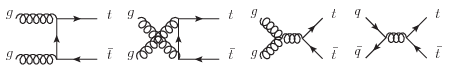
\includegraphics[width=0.8\textwidth]{fig/thry/fig_ttbar.png}
\caption{Feynman diagrams for \ttbar production at leading order QCD}
\label{fig:ttdiag}
\end{figure}

\begin{figure}
\centering
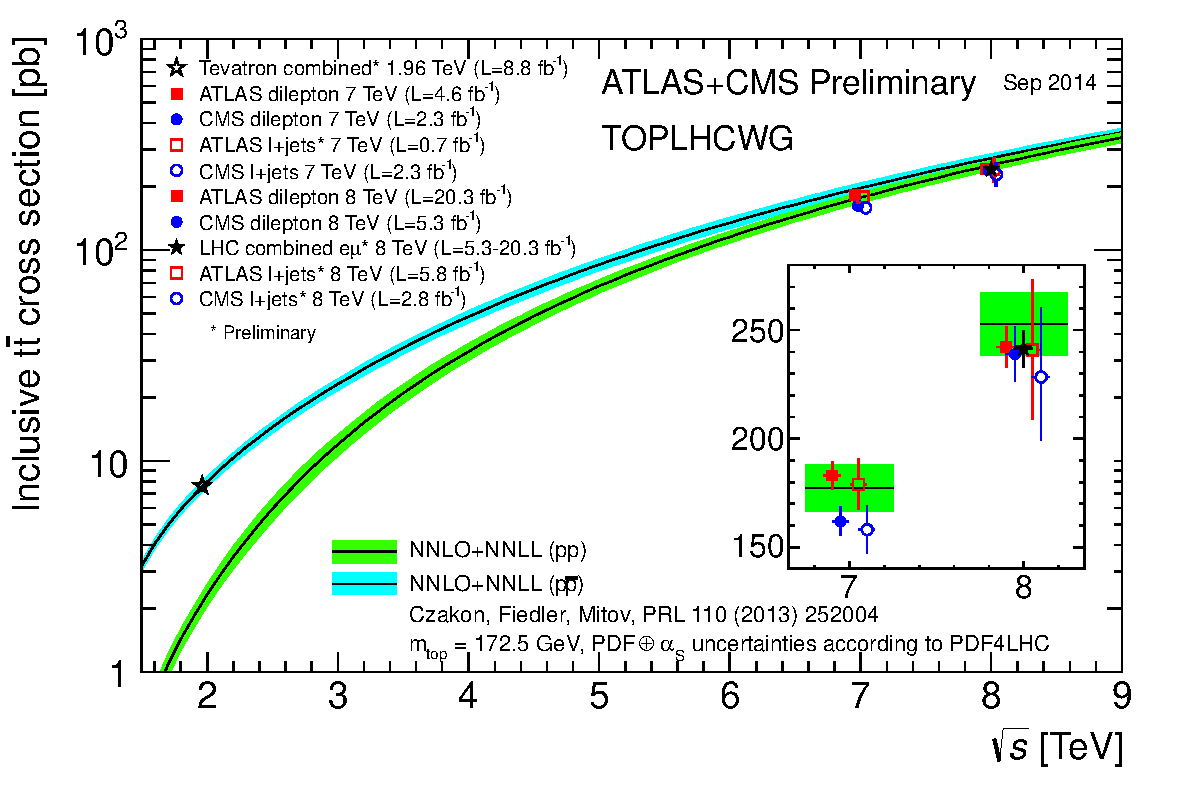
\includegraphics[width=0.8\textwidth]{fig/thry/tt_xsec_vsroots.pdf}
\caption{Summary of LHC and Tevatron measurements of the top-pair production cross-section as a function of the centre-of-mass energy compared to the NNLO QCD calculation complemented with NNLL resummation (top++2.0). The theory band represents uncertainties due to renormalisation and factorisation scale, parton density functions and the strong coupling. The measurements and the theory calculation is quoted at $m_{top}$=172.5 GeV. Measurements made at the same centre-of-mass energy are slightly offset for clarity.}
\label{fig:ttxsec}
\end{figure}

Top quarks can also be produced singly via electroweak processes. Because the weak coupling is much smaller than the strong coupling, fewer quarks are produced singly than in pairs. The Feynman diagrams for single top production are shown in Figure~\ref{fig:tdiag}. Single production can mediated by virtual $s$-channel and $t$-channel $W$-bosons. These production channels provide sensitivity to physics beyond the SM. Single tops are also produced in association with a $W$-boson ($Wt$-associated production). While negligible at the Tevatron, at the LHC, $Wt$-associated production provide a sizeable contribution to single top production. The inclusive cross-section for $s$-channel, $t$-channel and $Wt$-associated single top production has been computed to NNLO. This calculation is compared with the ATLAS experimental measurements of each channel in Figure~\ref{fig:txsec}.



\begin{figure}
\centering
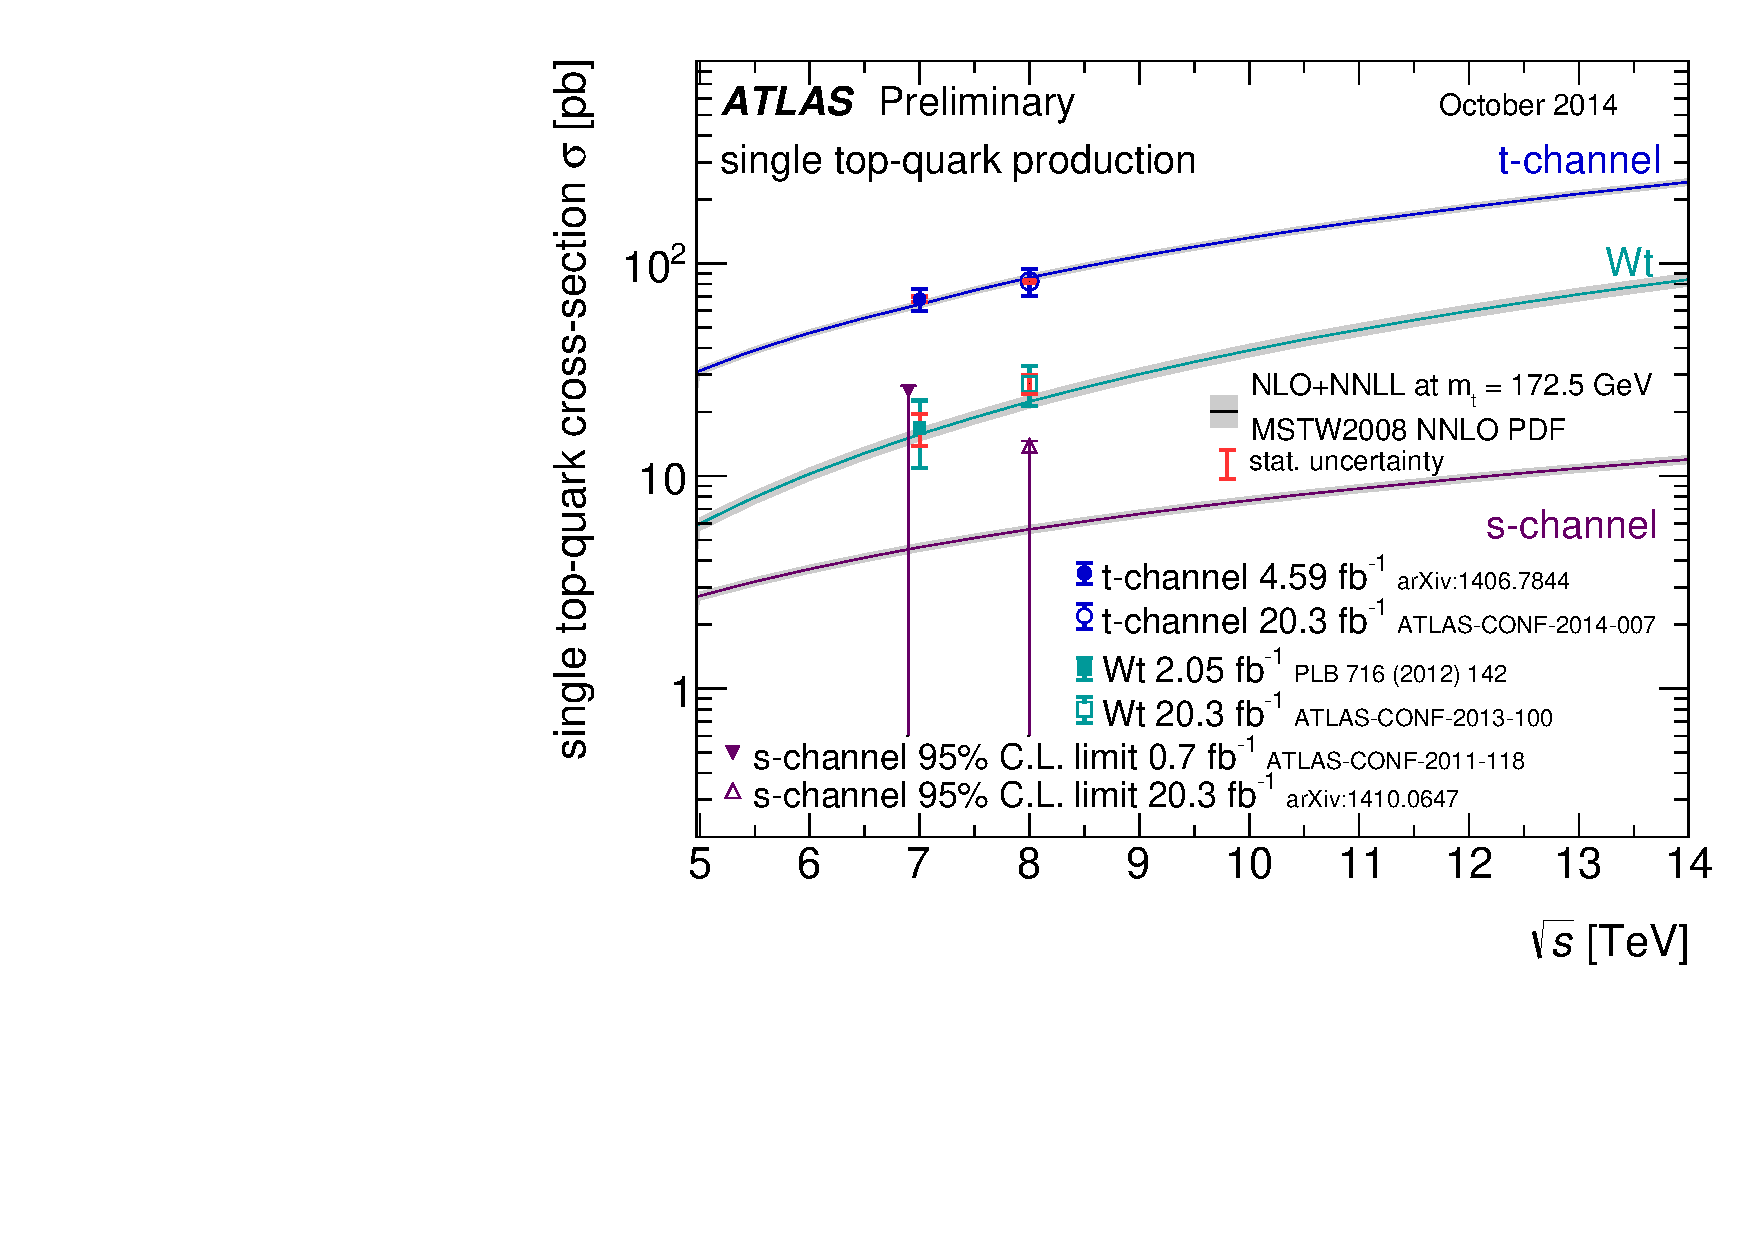
\includegraphics[width=0.8\textwidth]{fig/thry/singletop_allchanvsroots_ATLASonly.pdf}
\caption{Summary of ATLAS measurements of the single top production cross-sections in various channels as a function of the center of mass energy compared to a theoretical calculation based on NLO QCD complemented with NNLL resummation. For the $s$-channel only an upper limit is shown.}
\label{fig:txsec}
\end{figure}
\begin{figure}
\centering
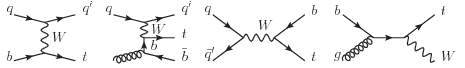
\includegraphics[width=0.8\textwidth]{fig/thry/fig_singletop.png}
\caption{Feynman diagrams for single top quark production at leading order QCD. From left to right: $t$-channel production as flavor excitation; $t$-channel production as $W$-gluon fusion; $s$-channel production; $Wt$-channel production.}
\label{fig:tdiag}
\end{figure}

\subsection{Top quark decays}
At lowest order in the SM, the top quark can only decay to a $W$ boson and a down-type quark: $t \rightarrow qW$ where $q=b,s,d$. The rate of each of these decays is proportional to the square of the Cabibbo-Kobayashi-Masakawa (CKM) matrix, $|V_{tq}|^2$. Measured from experiment, the CKM matrix governs quark mixing in flavor-changing weak decays~\cite{PDG}.

Weak hadron decays and the unitiary of the CKM matrix constrain the value of $0.9990 < |V_{tb}| < 0.9992$ at the 95\% C.L~\cite{Chetyrkin:1999ys}. Top quarks nearly always decay with $t \rightarrow Wb$.

Experimentally, the decay modes of \ttbar are distinguished by the decay of the two $W$-bosons:
\begin{description}
\item[All hadronic] Both $W$ bosons decay to quark pairs: $\ttbar \rightarrow WbWb \rightarrow bbqqqq$. Because there are 6 quarks in the final state, this channel has a large multi-jet background, which can be difficult to subtract. 

\item[Semi-leptonic] One $W$ boson decays to a quark pair and the other decays to a lepton and neutrino: $\ttbar \rightarrow WbWb \rightarrow bbqq \ell \nu$. This channel can be further categorized by lepton flavor.


\item[Dileptonic] Both $W$ bosons decay to leptons: $\ttbar \rightarrow WbWb \rightarrow bb\ell \nu\ell \nu$. Though the dilepton channel has the fewest events, it often provides least background.


\end{description} 

\section{Beyond the SM}
In addition to providing a test of the SM, the top quark may also provide a window to physics at higher energy scales beyond the SM.

The top quark is important in aesthetic problem with the Higgs mass known as the hierarchy problem or fine tuning. The Higgs mechanism provides an explanation for electroweak symmetry breaking and acquisition of mass by other SM particles. As a scalar particle, the Higgs receives higher-order corrections to its physical (measured) mass from interactions with fermions, gauge bosons and itself. These corrections are on the order of the Planck scale, $\mathcal{O}(\Lambda^2 \approx 10^{30-38} \gev)$, while the observed mass is class to the electroweak scale, $\mathcal{O}(100 \mev)$. Thus, in order to obtain the observed mass without introducing new physics, there must be an unnatural canceling. Since the dominant higher-order correction to the Higgs mass comes from the top, precisely measuring the top's mass and other properties may provide insight to this problem. 

In addition to the hierarchy problem, there are several other open questions which cannot be explained by the SM. The SM does not account for the 85\% of our universe made up of \textit{dark matter} particles, or provide an explanation for the observed asymmetry between matter and anti-matter. The SM also does not account for the observed non-zero mass of neutrinos or have a way to incorporate gravitational interactions.

Theorists have formulated many extensions to the SM that address these puzzles. Perhaps the most widespread, Supersymmetry (SUSY)~\cite{susy} proposes an additional superpartner for every particle in the SM. SUSY is especially popular because it naturally contains a light, stable, neutral dark matter candidate and solves the hierarchy problem. Diagrams from superpartners remove the need to fine tune the Higgs mass. Since SUSY has not been observed, the superpartners of SM particles must have different masses, and SUSY has to be a broken symmetry. However, in order to satisfactorily solve the hierarchy problem, the superpartners with the largest contributions to the Higgs mass must be $\mathcal{O}(\tev)$. This means that they should be discoverable at the LHC.

Another popular SM extension, called the Randall-Sundrum model~\cite{Lillie:2007yh}, posits an extra dimension in which gravity would propagate. This model includes a new particle, a Kaluza-Klein gluon, that propagates into the extra dimension and decays into a top quark pair.
%COULD ADD MORE ABOUT WHY SIGNALS IMPOR. See a thesis

Many of the signals for new physics are dominated by the top quark since heavier particles are more sensitive to higher energy scales.  The top pair production analyzed in this thesis is important as a background for \ttbar resonances~\cite{ATLAS-CONF-2015-009} and other searches~\cite{Aad:2014kra}.



% \section{QCD in hadron-hadron collisons}
% The protons collided at the LHC are composite objects made of point-like quarks held together by soft gluon emissions. Because of the asymptotic freedom of QCD, $\alpha_S$ is of order unity at the scale of these emissions within the proton, but as the scale of emissions increase $\alpha_S$ quickly drops. Then, at scales far above the QCD confinement scale ($\Lambda_{QCD} \sim 200$ MeV, the energy at which QCD because non-perturbative), the protons can be considered free objects. The hard scatter interaction with momentum transfer $Q$ occurs on a time scale that goes as $\tau \sim 1/Q$ which is much larger than the time scale of interactions between protons $\tau \sim 1/\Lambda_{QCD}$. This fact allows high energy proton collisions to be \textit{factorized} into two independent processes: the Parton Distribution Function (PDF), which describes the momentum distribution among the partons inside the proton and depends only on the momentum scale, and the partonic cross section $\hat{\sigma}$, which uses perturbative QCD to determine the calculates the scatter of the hard probe from one of the free partons inside the proton.

% PDF STUFF

% Then, the final \ttbar  cross section ($\sigma_{\ttbar}$) is a convolution of the partonic cross section ($\qqbar, qq \rightarrow \ttbar$)and the parton distribution functions (PDFs)~\cite{Moch:2008qy}:

% \begin{equation}
% \sigma_{\ttbar}(s, m_{t}) = \sum_{i, j} \int^1_0 dx_i  \int^1_0 dx_j f_i \left(x_i, \mu_F^2 \right) f_j\left(x_j, \mu_F^2 \right) \times \hat{\sigma}_{ij} \left( \hat{s}, m_{t}, \alpha_s \left(\mu_R \right), \mu_R,  \right)
% \end{equation}

% DISCUSSION OF GLUON GLUON ETC AT LHC

% At the LHC, $qg$ scattering occurs with the highest parton luminosity but the partonic cross-section $\hat{\sigma}_{qg}$ is smaller than either $\hat{\sigma}_{gg}$ or $\hat{\sigma}_{qq}$. The largest contribution for top pair production at the LHC comes from gluon-gluon fusion, due to the combination of a large partonic cross-section and the second largest parton luminosity. The second largest contribution comes from quark-antiquark annihilation. At NLO QCD, the total \ttbar\ production at the LHC comprises approximately 90\%

% At the Tevatron, a previous $p\bar{p}$ collider with lower energy, \ttbar production was 

% AHHH REPETITIVE









